\documentclass[conference, a4paper]{IEEEtran}
\usepackage{blindtext, graphicx}

\usepackage{caption} 
\captionsetup[table]{skip=8pt}

\begin{document}

\title{ID2010 Lab 2 - Tag}


\author{\IEEEauthorblockN{Andreas Hallberg}
\IEEEauthorblockA{KTH Royal Institute of Technology\\
CINTE2010 / TSEDM 2013\\
Email: anhallbe@kth.se}}
\maketitle

\IEEEpeerreviewmaketitle


\section{Introduction}
This report describes how I implemented the game of Tag. The game consists of a number of rooms (Bailiffs), the Bailiffs are contained in separate JVM instances. Each Bailiff serves as an execution environment for mobile agents (the Players). A player has two states: \textbf{it} and \textbf{not it}. At any given time there can only be one \textbf{it} player, which I will refer to as a \textbf{tagger}. The purpose of the tagger is simple; tag others, i.e pass the \textbf{it} property to another player. The player can only tag another player if they both reside in the same Bailiff. So the tagger needs to find a populated Bailiff, move to it, and try to tag someone. The non-tagger players simply need to avoid the tagger, i.e avoid bailiffs where the tagger is present.

\section{Player strategy}
The strategy of the players is depicted in Fig. \ref{player-strategy}:
\begin{figure}[h!]
	\centering
	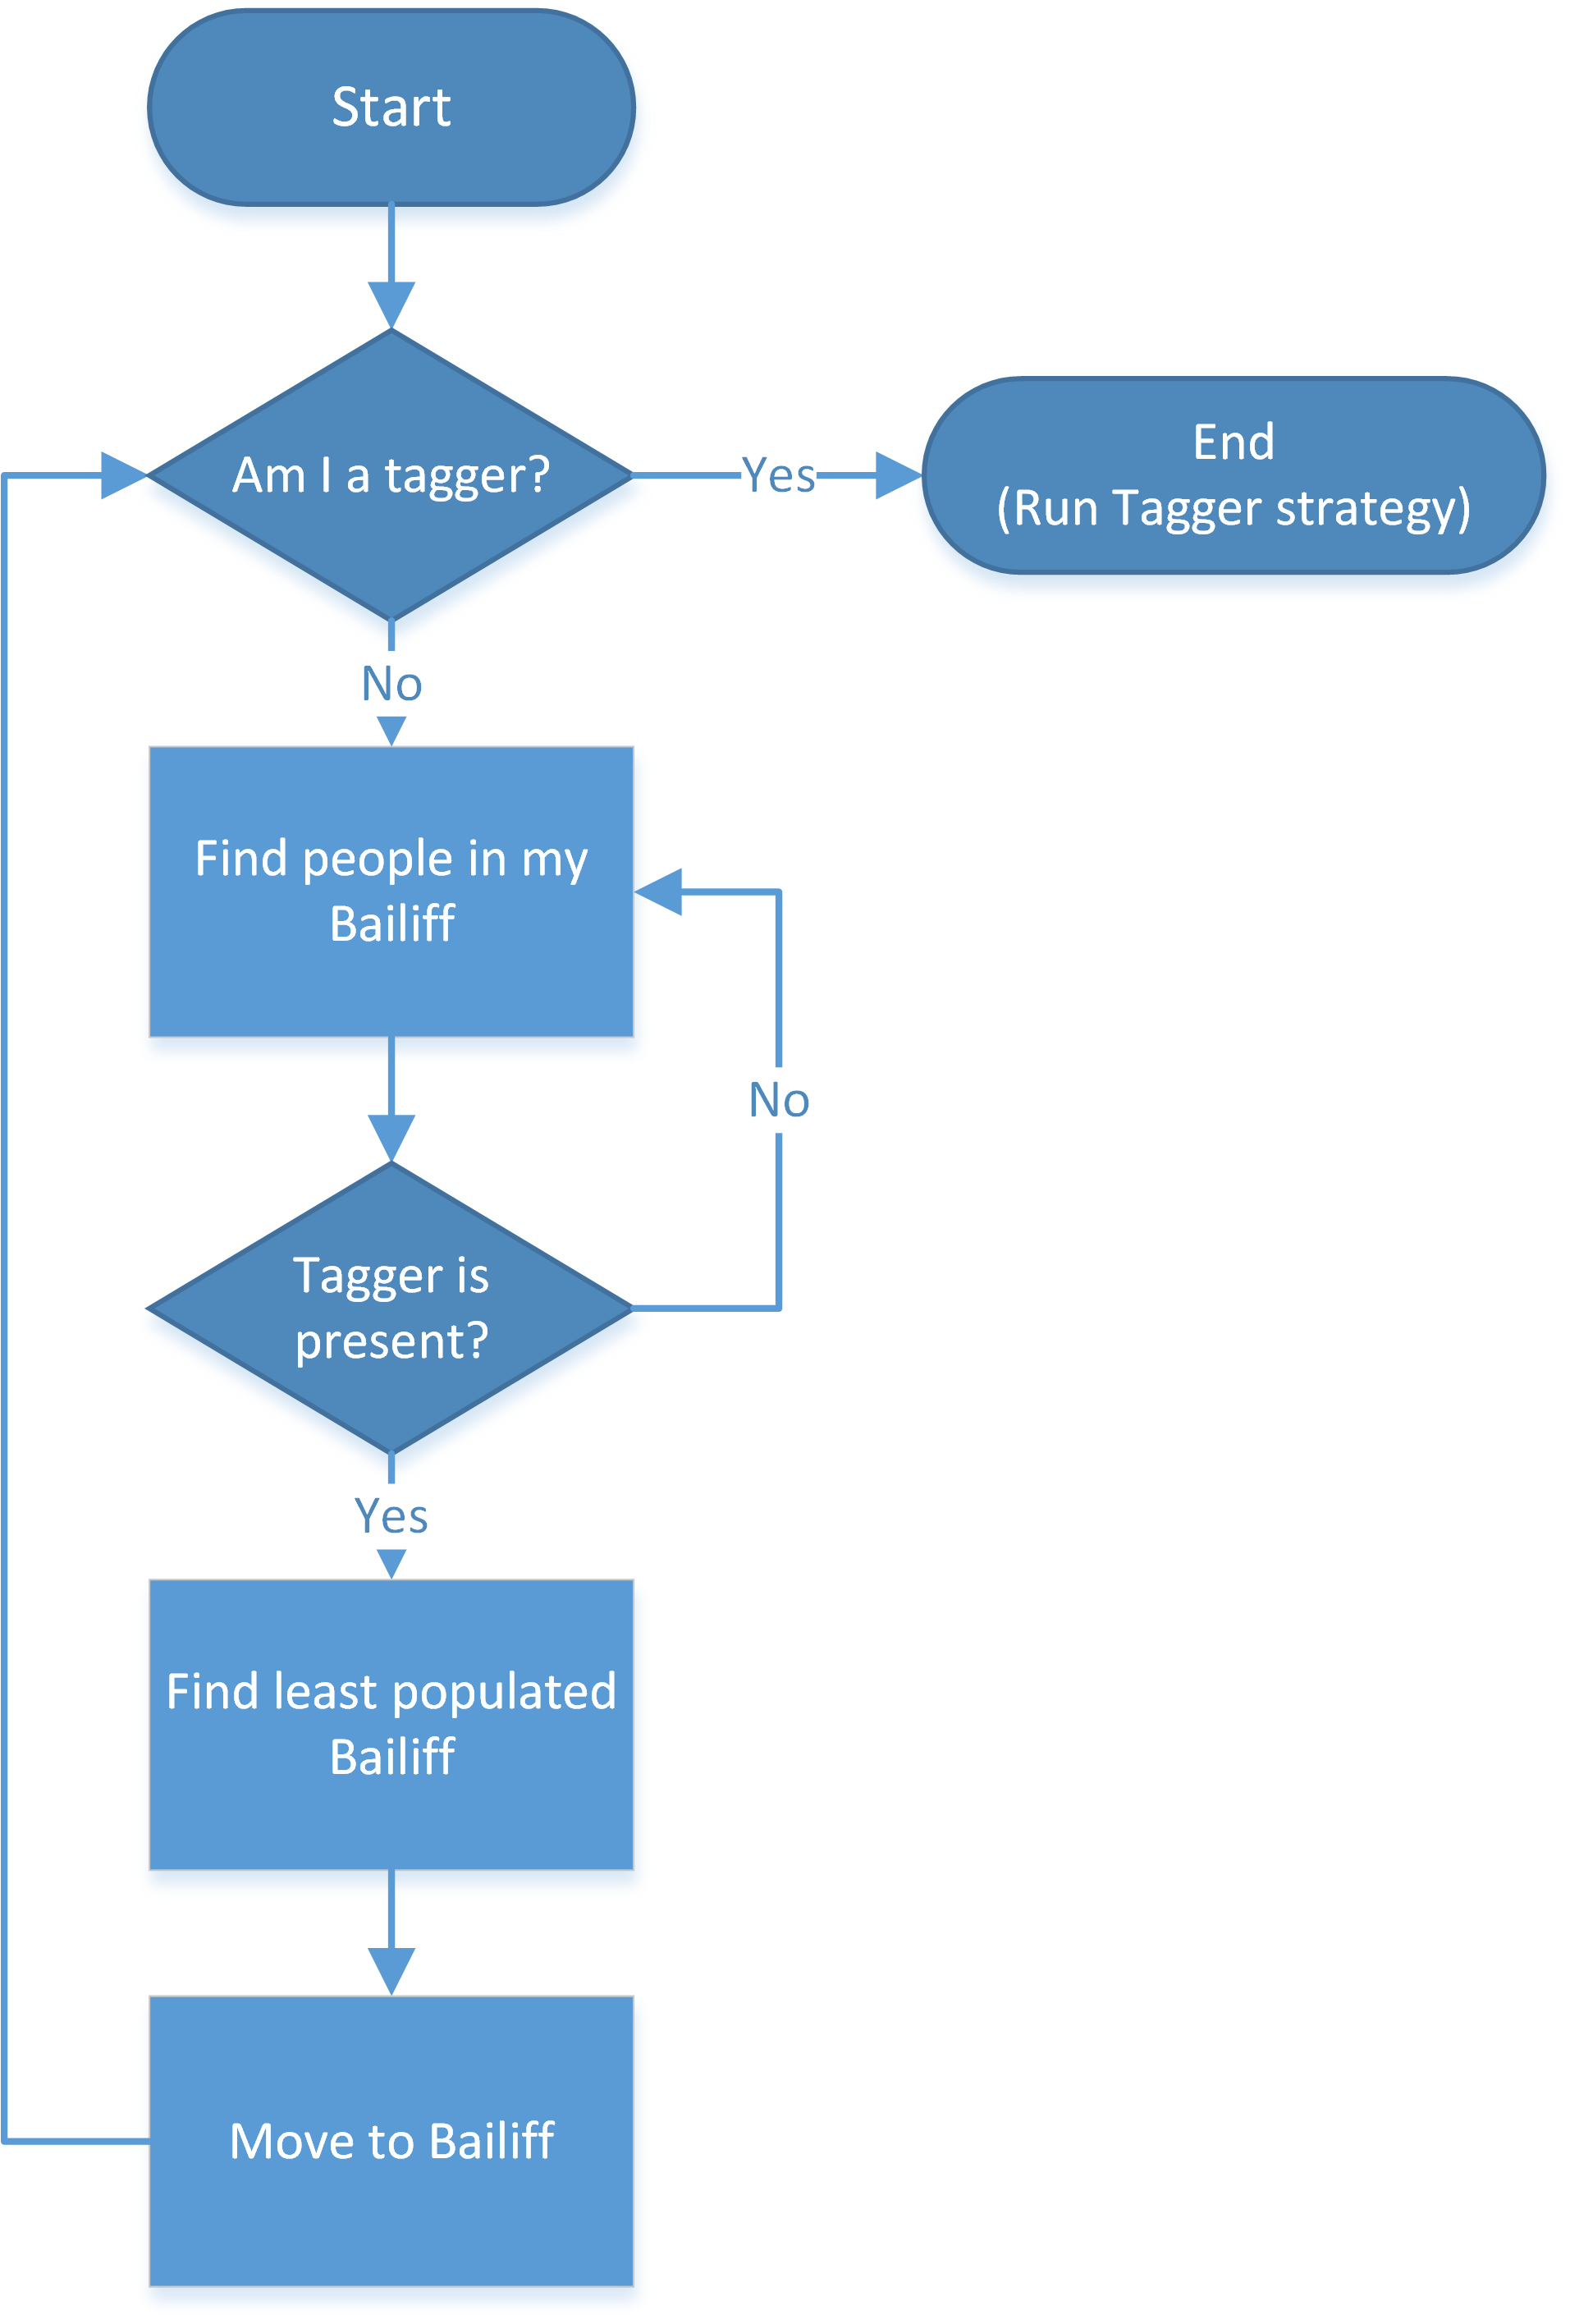
\includegraphics[scale=0.8]{player-strategy}
	\caption{The player strategy. The player will not move unless the tagger is present. It will run away to the least populated Bailiff once the tagger arrives, since that one is least likely to be the next target of the tagger.}
	\label{player-strategy}
\end{figure}


\section{Tagger strategy}
The following is the strategy of the Tagger agent (Fig. \ref{tagger-strategy}):
\begin{figure}[h!]
	\centering
	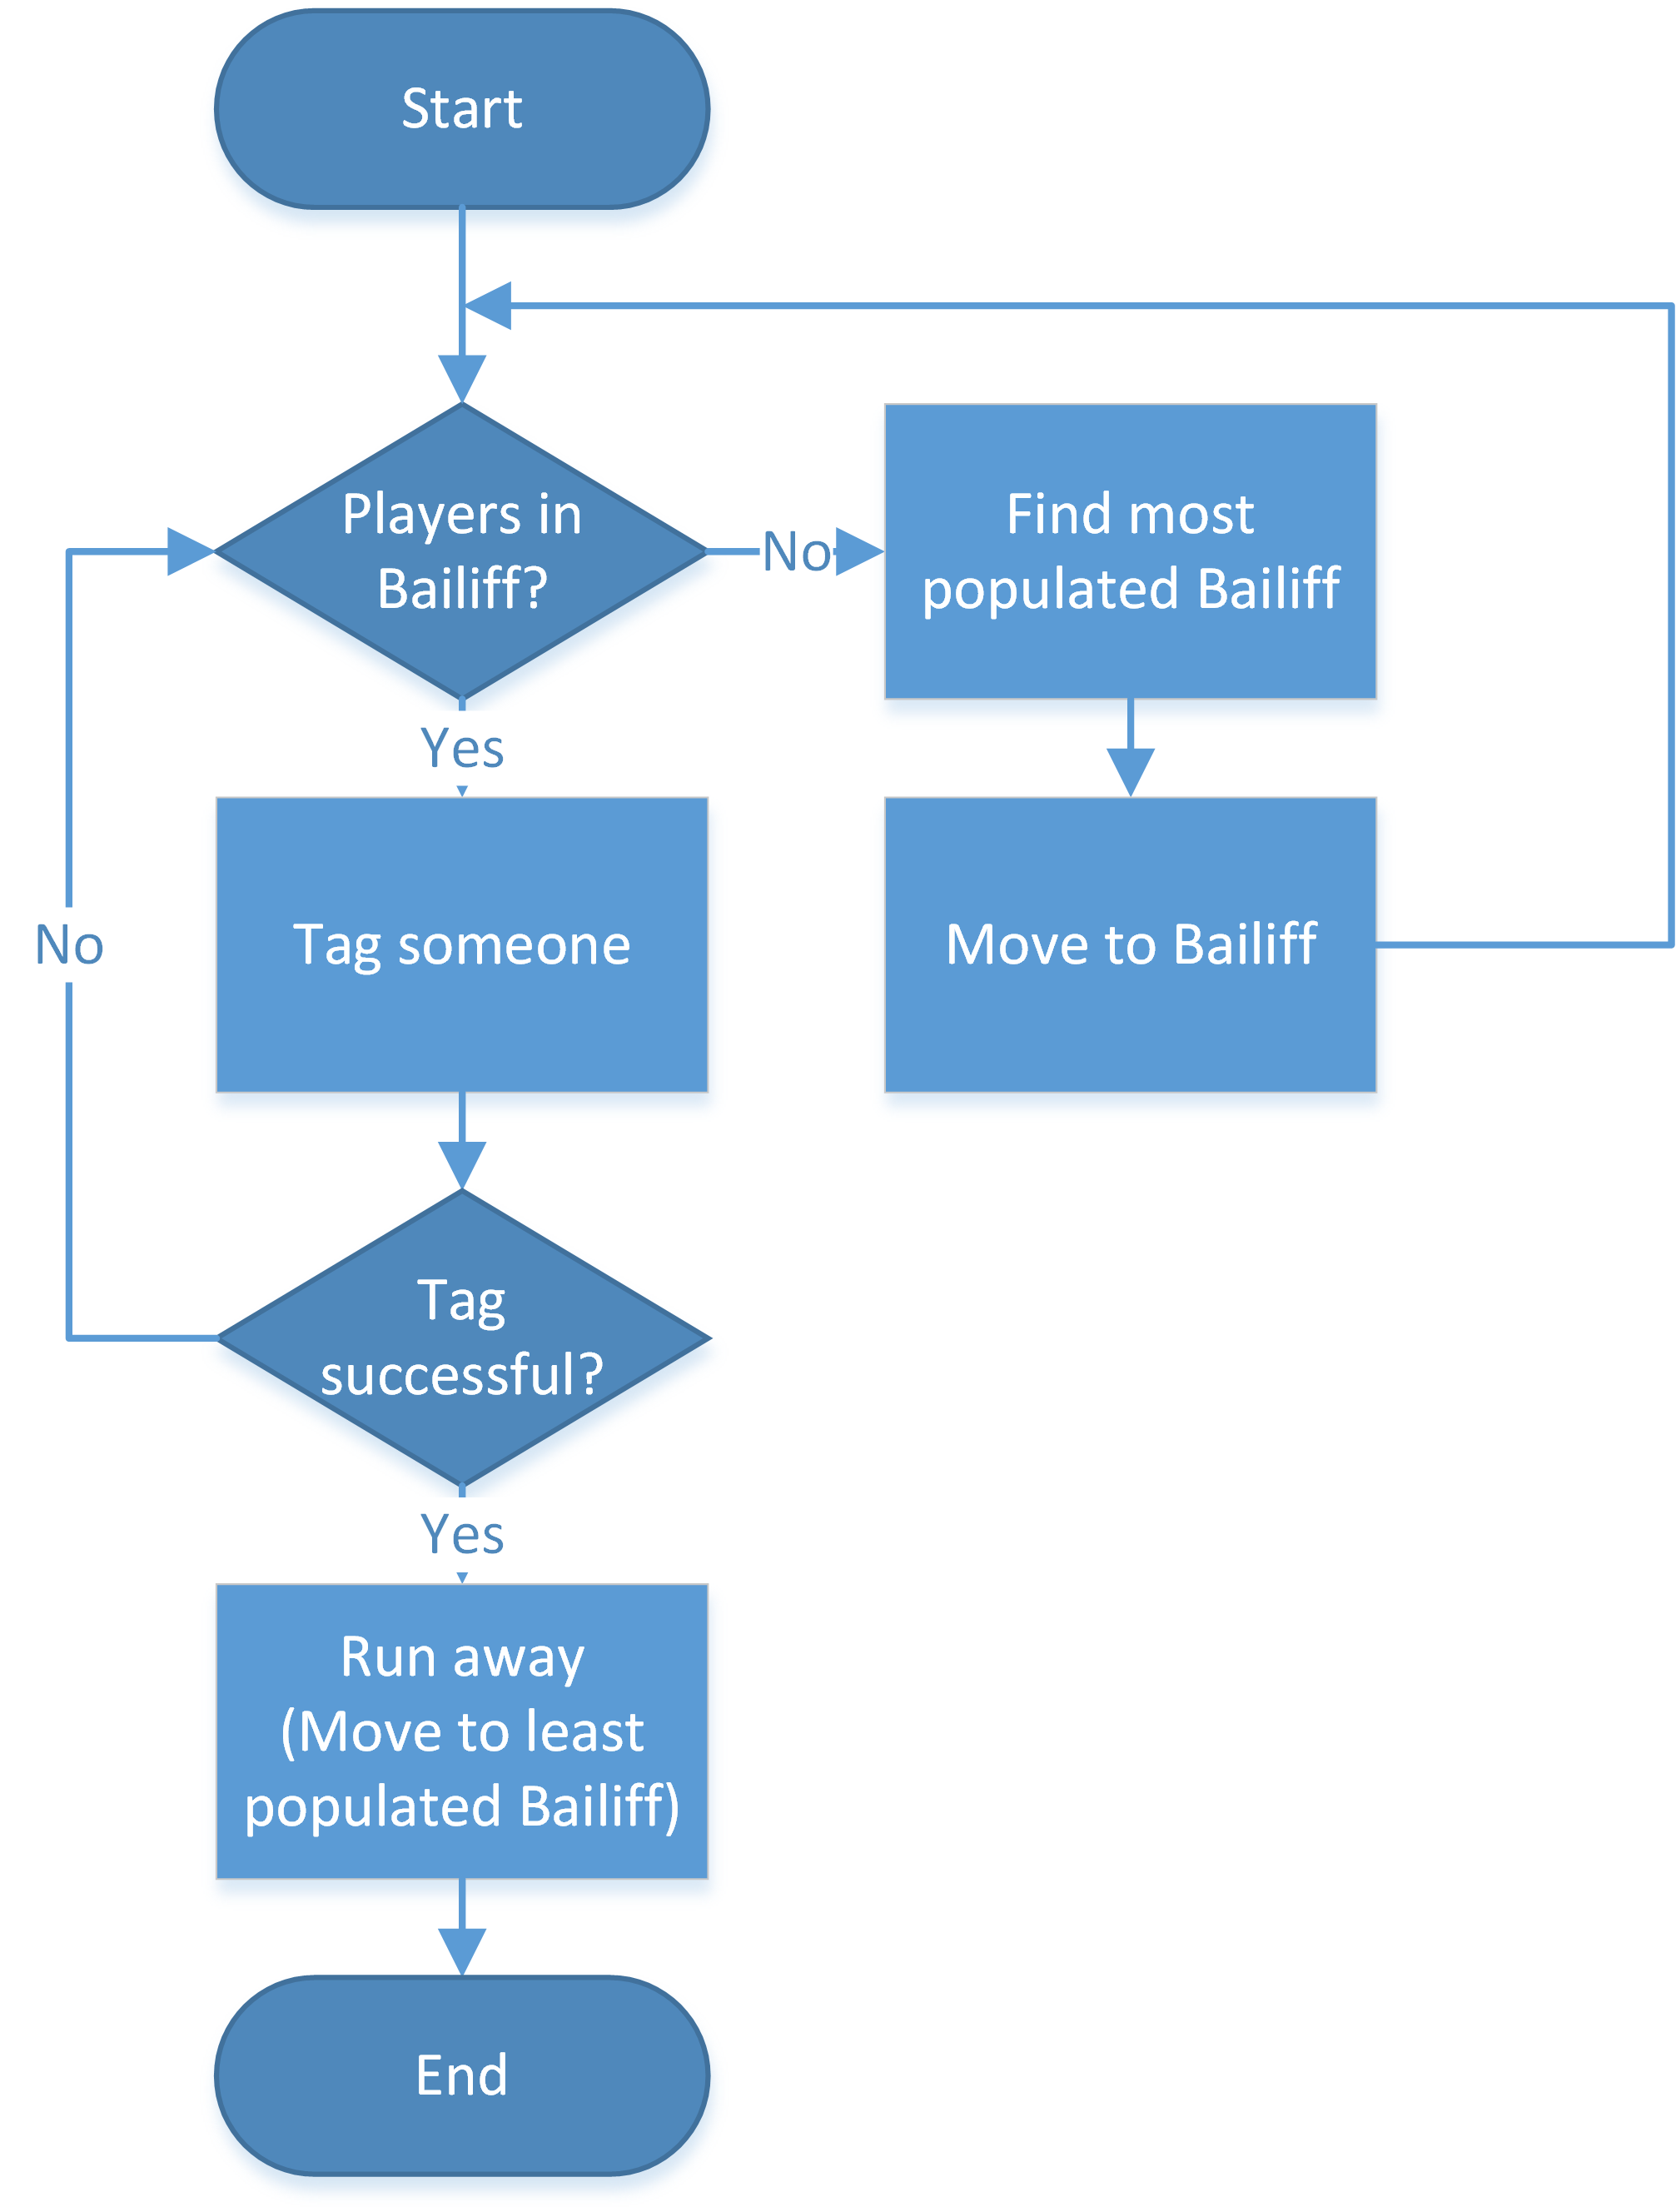
\includegraphics[scale=0.9]{tagger-strategy}
	\caption{Strategy of the Tagger. Once it has successfully tagged someone else it is now a target for the new tagger, so it needs to run to another room (essentially using the same strategy as the other non-taggers).}
	\label{tagger-strategy}
\end{figure}

\section{Agent-to-Agent communication}
Agents (players) do not speak directly to each other due to the nature of the Jini system and their high mobility. Instead they use the Bailiffs as proxies. The following methods were added to the Bailiff interface:
\begin{center}
\begin{verbatim}
/**Get a list of players in this bailiff**/
  List<UUID> playersInBailiff()
    
/**Ask if a player is the tagger**/
  boolean    isIt(UUID name)
    
    
/**Tag a player**/
  boolean    tag(UUID name)
    
/**Get the name of this bailiff**/
  String     getRoomName()
\end{verbatim}
\end{center}
A Bailiff keep track of its players in a Map, where the players are referenced by their name (UUID). The players are added/removed from the map whenever it migrates to/from the bailiff. Threads (players) will access the map concurrently, so \textit{java.util.concurrent.ConcurrentHashMap} is used to prevent any complications with concurrent reads/writes.

\section{User Interface}
The UI is a combination of graphical- and command line interface. The Bailiff GUI displays a number that presents the number of players currently in the bailiff. If the Tagger is present the number is displayed with a red font. The GUI can be seen in Fig. \ref{fig010} - \ref{fig111}. The CLI will display when a player is tagged, as well as other useful output when the -debug flag is provided.

\section{Program execution}
The following figures depict the Bailiff GUI during a game of Tag with 3 bailiffs and 3 players. First the 3 bailiffs are started with \textit{./bailiff.sh -room rX}. Then the players are started one by one with \textit{./player.sh}. The last player is started with the \textit{-it} argument to indicate that it should be the tagger at start. The game goes on and the players keep tagging each other until the program is manually terminated.
\begin{figure}[h!]
	\centering
	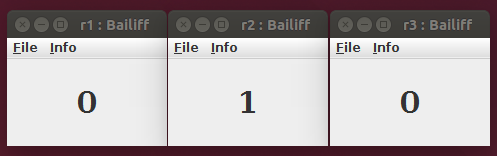
\includegraphics[scale=0.4]{010}
	\caption{Player1 joins. No reason to do anything.}
	\label{fig010}
\end{figure}

\begin{figure}[h!]
	\centering
	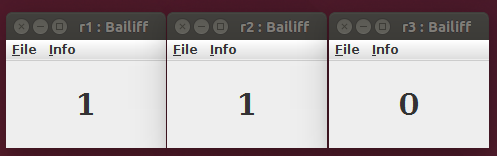
\includegraphics[scale=0.4]{110}
	\caption{Player2 joins. Still no reason to move.}
	\label{fig110}
\end{figure}

\begin{figure}[h!]
	\centering
	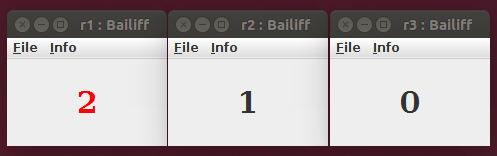
\includegraphics[scale=0.4]{210.png}
	\caption{Player3 (it) joins the same bailiff as Player2. Player3 will try to tag Player2, and Player2 will try to run to the empty bailiff.}
	\label{fig210}
\end{figure}

\begin{figure}[h!]
	\centering
	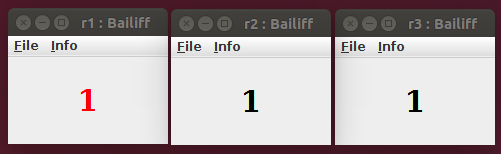
\includegraphics[scale=0.4]{111}
	\caption{Player3 managed to tag Player2 and ran away, or Player2 managed to run away. In either case "it" is now alone in Bailiff 1.}
	\label{fig111}
\end{figure}

\section{Conclusion}
The program successfully plays the game of Tag with multiple Bailiffs and players. I haven't handled all the possible errors such as incorrect use of the UI, as that is outside the scope of this assignment. If for instance a bailiff is terminated without using the "exit" button in the GUI, there are no guarantees that the game will go on. If the tagger is currently inside the incorrectly terminated Bailiff, there is no procedure to automatically make another player the tagger.

There are some complications with the GUI when the program is run with a larger number of agents. The number of players displayed in each bailiff may be incorrectly updated, but the game does seem to execute correctly according to the command line output.

\end{document}


